\section{Results}
In total 498 test cases were executed, totalling 24,900 packet transmissions. Of this total 19,545 were successfully received (78.5\%). The distribution of receive conditions for these individual points is indicated by Figure \ref{fig:density_plot}. Note that the raw \ac{rssi} values returned by the Radiohead library, and therefore the datalogger, are in fact packet strength for the SX1276 module; therefore a post-processing step has been applied to get separate packet strength and \ac{rssi} values valid for the RFM95W module. For each test definition executed, the log-mean and log-standard deviations of the successfully received packet's: \ac{rssi}, \ac{snr}, and strength have been calculated.
\begin{figure}[H]
    \centering
   	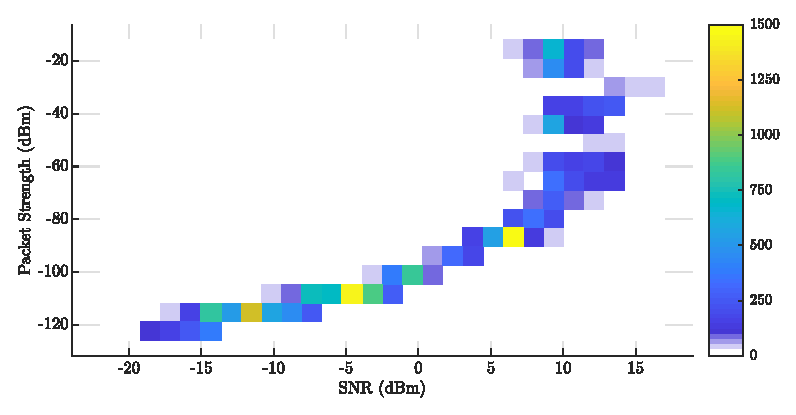
\includegraphics{Figures/density_plot}
    \caption[Test data distribution plot]{
    Density plot of received packet transmissions modelled as a bi-variate histogram with colour indicating received packet count. \\$Total\enskip Points = 19,545$
    }
    \label{fig:density_plot}
\end{figure}

\section{Discussion}
Some writing
\subsection{PHY Layer Performance}

\subsubsection{Spreading Factor}

\subsubsection{Coding Rate}

\subsubsection{Packet Length}

\begin{figure}[H]
    \centering
   	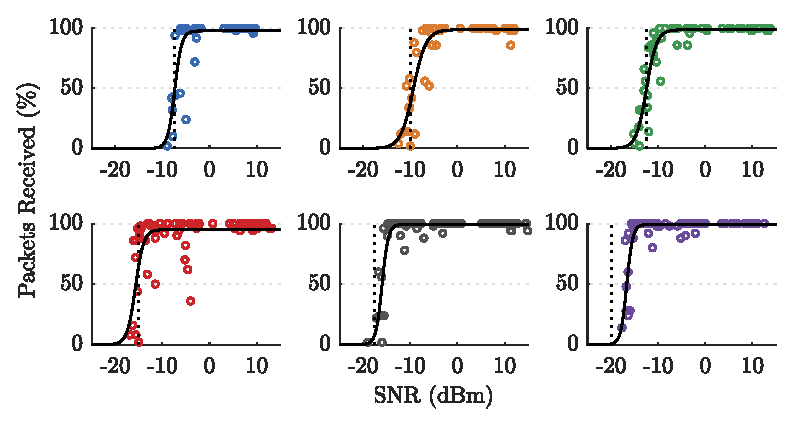
\includegraphics{Figures/snr_pp_separate_plot}
    \caption[Plots of \ac{snr} vs Packet Receive Percentage]{
   \ac{td} mean \ac{snr} values plotted against their packet receive percentages, separated by \ac{sf}s (Order = [[7, 8, 9], [10, 11, 12]]). For each \ac{sf} plot: the theoretical demodulation limit is indicated by the dotted line and the solid line corresponds to the best-fit sigmoid function; these are repeated in Figure \ref{fig:sf_pp_fit}. Although the best-fit sigmoids give a good representation of the general data pattern, and provide empirical demodulation cut-offs, they do not capture the high-variance receive behaviour when approaching the cut-off. This is reflected by the fact that only 62\%, 60\%, 66\%, 39\%, 77\% and 82\% of the respective training points fall inside the corresponding 95\% confidence interval. Notably \ac{sf}10 has very high-variance; this is reflected in the 95\% maximum receive chance. 
    }
    \label{fig:snr_pp_separate}
\end{figure}

\begin{figure}[H]
    \centering
   	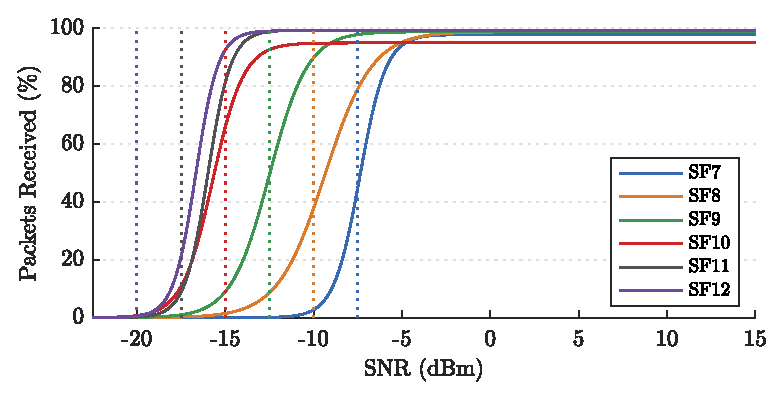
\includegraphics{Figures/sf_fit_plot}
    \caption[Plot of sigmoid best-fits for \ac{snr} vs Packet Receive Percentage]{
    Plot of sigmoid best-fits generated in Figure \ref{fig:snr_pp_separate}. The plot clearly demonstrates the positive effect increasing \ac{sf} has on demodulation performance of the receiver. For \ac{sf}=7,8,9,10 demodulation success starts dropping approximately 2.5dBm before the theoretical limit ($D_L$), with a 50\% packet receive chance at $D_L$. This holds less so for \ac{sf}=11, for which drop-off starts around $D_L - 5dBm$, until $D_L$ where there is only a 10\% receive success. For \ac{sf}=12 drop-off starts around $D_L - 7.5dBm$, until $D_L$ where there is a 0\% receive success. Given that \ac{rssi} was relatively stable when $\ac{snr} < 0$, and that expected performance holds until a certain \ac{snr}, there is an indication that the sensitivity of the receiver is not as high as stated. 
     }
    \label{fig:sf_pp_fit}
\end{figure}

\subsection{Environmental Effects}
\subsubsection{Open (Free) Space}
High noise floor indicates that either the receiver's noise figure is not correct or there is more noise than expected in the environment. The fact that demodulation limit is nowhere near the true limit for SF10 onwards suggests that the cheaper radio does not perform correctly.
\subsubsection{Forest}
\subsubsection{Radio Height}
Increasing radio height massively increased range once reached 1m

% Distance in relatively open space (got)
% Distance in trees (got)
% Closeness to ground (got)
% Coding rate ??? (sort of got)
% Difference in slight movements (!!!)
%Lessons Learnt 
https://www.thethingsnetwork.org/forum/t/no-lower-rssi-than-121-dbm-possible-in-ttn/19890/15